\documentclass[aspectratio=169]{beamer}

\usetheme[titleformat=allcaps,sectionpage=simple,progressbar=frametitle,background=dark]{metropolis}
\RequirePackage{etoolbox}
\RequirePackage{ifxetex}
\RequirePackage{ifluatex}
\RequirePackage{pgfopts}

\usepackage{color}
\definecolor{background}{HTML}{ffffff}
\definecolor{text}{HTML}{333333}
\definecolor{background}{HTML}{333333}
\definecolor{text}{HTML}{ffffff}
\definecolor{warning}{HTML}{f0ad4e}
\definecolor{success}{HTML}{5cb85c}

\setbeamercolor{progress bar}{fg=success,bg=background}
\setbeamercolor{progress bar in section page}{fg=success,bg=background}
\setbeamercolor{title separator}{fg=warning,bg=text}
\setbeamercolor{normal text}{fg=text,bg=background}
\setbeamercolor{frametitle}{fg=text,bg=warning}
\setbeamercolor{section title}{fg=text,bg=warning}
\setbeamercolor{palette primary}{bg=warning}

\setbeamercolor{titlelike}{fg=text}
\setbeamercolor{author}{fg=text}
\setbeamercolor{date}{fg=text}
\setbeamercolor{institute}{fg=text}

%\usepackage{default}
\usepackage{graphicx}
\usepackage{amssymb}
\usepackage[ngerman,english]{babel}
\usepackage{appendixnumberbeamer}
\usepackage{textcmds}
\usepackage{float}
\usepackage{csquotes}

\usepackage{pgfpages}
%\setbeameroption{show notes on second screen}

% Define block styles
\tikzstyle{decision} = [diamond, color=background, fill=red!20, text width=5em, text badly centered]
\tikzstyle{block} = [rectangle, color=background, fill=blue!20, text width=7em, text centered, rounded corners, minimum height=4em, text centered]
\tikzstyle{cloud} = [ellipse, color=background, fill=green!20, minimum height=2em, text centered, text width=4em]

\title{Interpolation - On the example of the intra-urban Heat island effect in Berlin}
\subtitle{FOSSGIS Seminar}
\date{February 3, 2021}
\author{Anja Doppelmayr (3673519) \& Malte Heinzelmann (3293437)}
\institute{Ruprecht-Karls-Universit\"at Heidelberg}

\makeatletter
\def\beamer@framenotesbegin{% at beginning of slide
	\usebeamercolor[fg]{normal text}
	\gdef\beamer@noteitems{}%
	\gdef\beamer@notes{}%
}

\setlength{\metropolis@titleseparator@linewidth}{2pt}
\setlength{\metropolis@progressonsectionpage@linewidth}{2pt}
\setlength{\metropolis@progressinheadfoot@linewidth}{2pt}

\newlength\beamerleftmargin
\setlength\beamerleftmargin{\Gm@lmargin}
\makeatother

\usepackage[export]{adjustbox} 

\usepackage{tikz}
\usetikzlibrary{arrows,positioning,shapes,arrows.meta}

\usepackage[absolute,overlay]{textpos}
\setlength{\TPHorizModule}{\paperwidth} % horizontal unit
\setlength{\TPVertModule}{\paperheight} % vertical unit

\usepackage[
backend=biber,
style=alphabetic,
]{biblatex}
\usepackage{tabularx}
\usepackage{pifont}% http://ctan.org/pkg/pifont

\newcommand{\cmark}{\ding{51}}%
\newcommand{\xmark}{\ding{55}}%

\addbibresource{../writeup/biblatex.bib} %Imports bibliography file

\newenvironment*{env}{}{}

\begin{document}
	\begin{frame}[plain]
		\makebox[0pt][l]{%
			\hspace*{-11mm}
			%\hspace*{-\beamerleftmargin}
			\raisebox{-\totalheight}[0pt][0pt]{%
				\includegraphics[width=\paperwidth,keepaspectratio]{images/background}
			}
			\hspace*{-\paperwidth}
			\hspace*{-4.5mm}
			\raisebox{-\totalheight}[0pt][0pt]{%
				\includegraphics[width=\paperwidth,height=\paperheight]{images/backdrop.png}
			}
		}
		\begin{textblock}{1}[1,1](0.995,0.99)
			\setlength\topsep{0pt}
			\begin{flushright}
				\tiny\color{text} Source: Pixabay (davidph, topography-station-measurement-202278)%
			\end{flushright}
		\end{textblock}
		\titlepage
	\end{frame}

	\begin{frame}{Agenda}
		\tableofcontents[]
	\end{frame}

	% !TeX root = ../document.tex

\section{Introduction}

The basic definition of an urban heat island (UHI) effect is \ldq{}[...] that an urban area or metropolitan area is significantly warmer than its surrounding rural areas due to human activities\rdq{} \cite{takebayashi_chapter_2020}. Higher temperatures than those in the surrounding areas can indicate heat islands. As known, infrastructure such as buildings, roads, etc. absorb and re-emit the sun’s radiation in the form of heat, whereas natural landscapes such as forests and water bodies have a cooling effect. \cite{us_epa_learn_2014}

Thus, replacing natural areas with dense concentrations of buildings, infrastructure, pavements and other sealed surfaces that absorb and retain heat, leads to an increase in air temperature in urban areas relative to their rural counterparts. This effect, however, is not only comprehensible when comparing a metropolitan area to its surrounding, more natural realm, but also within a city itself. 

Temperature differences within urban areas are so-called \ldq{}Intra-Urban Heat Islands (IUHI)\rdq{}. \cite{bruns_stable_2017}
These heat islands within the city have a negative effect, not only for people’s health, well-being and comfort - especially in regard to the vulnerable population – but also for infrastructure, urban ecosystems and the living environment. Moreover, increased heat stress has been found to be the source for higher energy demands (for cooling) and the degradation of air quality in urban areas. \cite{mohajerani_urban_2017}

\subsection{Project Goals}

The fundamental aim of our study is to analyze temperature data in order to be able to create a visual product of the intra-urban heat islands effect, by making this effect and it's development throughout the day visible. Subsequently, the final animation can be used to support planning authorities. Current developments in regard to climate change urge the implementation of countermeasure as well as mitigation strategies in urban areas, where more greening is obviously needed. \cite{ketterer_comparison_2015}

Fostering measures such as cool and reflective pavements, green spaces and air circulation systems \cite{mohajerani_urban_2017} can be supported by preparing material, which helps to identify areas of increased heat stress and evaluated where countermeasures need to be implemented.

Our approach, therefore, includes the comparison of changes in air temperature over the course of the warmest day in 2019 (25.7.) and 2020 (9.8.) in Berlin. The study area is defined by Germany’s capital city Berlin. This site was chosen due to the availability of various data points and measurements in regard to our main source of data: openSenseMap (see section \ref{sec:data}). Furthermore, we hope to find a more significant intra-urban heat islands effect, as compared to other areas in Germany, merely because of the size and a relatively high degree of sealed surfaces. \cite{gdv_munchen_2018} Although the effect should be identifiable in similar urban areas, the comparison of different interpolation methods stands in the focus of this project, which is why we decided to use a more self-evident study site. Thus, the result of the comparison of the different methods below should point towards one overall method, which is best-suitable for answering questions in relation to the IUHI effect. 

\subsection{Data: Selection and preparation (workflow)}
\label{sec:data}

Typically, the UHI effect is measured by the temperature difference between a city and its surrounding area.\cite{us_epa_learn_2014} In a study from 2012, the authors used land use/land cover, soil texture, and a digital elevation model as independent variables for interpolating and predicting temperature data in an area with a limited number of stations.\cite{samanta_interpolation_2012} As our study site did show various stations where temperature was measured on a regular basis, we were able to use this data directly and were hence not dependent on predicting point data based on independent variables. While our data did not demand for a series of different factors, but accurate and \ldq{}clean\rdq{} temperature data, the main preparation work was dedicated to extracting useful data, averaging the temperatures and selecting relevant sensor types (discussed below). Consequently, our temperature data is limited by the ultimate measurements of the different stations, their reliability and accuracy, which can be influenced by immediate surroundings or technical failure (also discussed in section \ref{sec:discussion}). Thus, if we would bring different variables, like elevation, solar radiation, wind speed and direction, distance to natural (vegetated and water) and artificial surfaces etc. into play, then the results and statements could be more accurate. With respect to time and thematic priority, this would, however, be outside the scope of this project.

Due to the fact, that openSenseMap is a citizen science project, not all stations will provide data of equal quality. The question, if temperature data derived from openSenseMap alone is representative for visualizing IUHI, is also a question of selecting a specific time-frame. Our central goal is to use the methods of interpolation to show local temperature variations and - after further analysis - be able to identify areas with higher concentrations of heat stress. The end product is aimed at generating an animation of these results. Based on these objectives and the fact that an analysis of temperature variability over a longer period of time would require large amounts of data, we decided to focus on the daily variation of the IUHI for the two selected days within the last two years, as mentioned before.

For the preparation of the data sets we had to take a few preliminary steps and explore the data at hand. For this purpose, we downloaded raw data from \url{https://opensensemap.org/} and aggregated the temperature data for the hottest day of the year 2019 and 2020, the 25.07 and 09.08 respectively. The initial number of stations downloaded from opensensemap.org resulted in 86 for 2019 and 121 for 2020 respectively. However, as some stations lacked data values for the necessary (10-minute-average) time intervals of the selected days, these had to be filtered. In a next step, a selection was made based on the double standard deviation – outliers were removed and the final data set consisted of 73 and 88 stations.

Furthermore, the sensor descriptions posed a problem as the type of measurement is a free-text field, thus allowing contributors to specify the type freely. The API endpoint (\url{/boxes/data}) requires the user to specify a phenomenon name within the request. Therefore, only the most common name \ldq{}Temperatur\rdq{} was used.

The final product used for further analysis consisted of a collection of stations and their aggregated measurements for each day.


\begin{figure}[b!]
	\centering
	\scalebox{0.85}{
		\begin{tikzpicture}[node distance = 2cm, auto, every node/.style={color=text, fill=background, font=\sffamily}, align=center]
			% Place nodes
			\node [block] (in) {openSenseMap};
			\node [cloud, right=1.6cm of in, text width=7em] (avg) {Average\\into 10 minute intervals};
			\node [cloud, right=1.6cm of avg, text width=8em] (filter) {Filter\\by std deviation};
			\node [decision, below=1.6cm of filter] (interpolate) {Interpolate};
			\node [cloud, left=1.6cm of interpolate, text width=8em] (colorize) {Colorize\\1-band Tiff $\Rightarrow$ 4-band RGBA Tiff};
			\node [block, below=2.3cm of in] (out) {Generate frame};
			% Draw edges
			\draw [->] (in) -- (avg);
			\draw [->] (avg) -- (filter);
			\draw [->] (filter) -- (interpolate);
			\draw [->] (interpolate) -- (colorize);
			\draw [->] (colorize) -- (out);
		\end{tikzpicture}
	}
	\caption{Project workflow overview}
	\label{fig:workflow}
\end{figure}




	\include{content/interpolation}
	
	\include{content/project}
	
	% !TeX root = ../document.tex

\section{Results}

Within this section we will present the differences in the results of the aforementioned interpolation methods and different implementations. For reference figure \ref{fig:result_berlin} shows all stations used in the following images, their respective temperature on the 9th August 2020at 12:00 and the surface class according to OpenStreetMap data.

The results will be analyzed by visual differences and overall level of accuracy towards the research question. First, we are going to take a look at the visual differences and compare the resulting images of the different interpolation methods, as well as the results of the same methods calculated with the help of different FOSSGIS implementations.

\begin{figure}[H]
	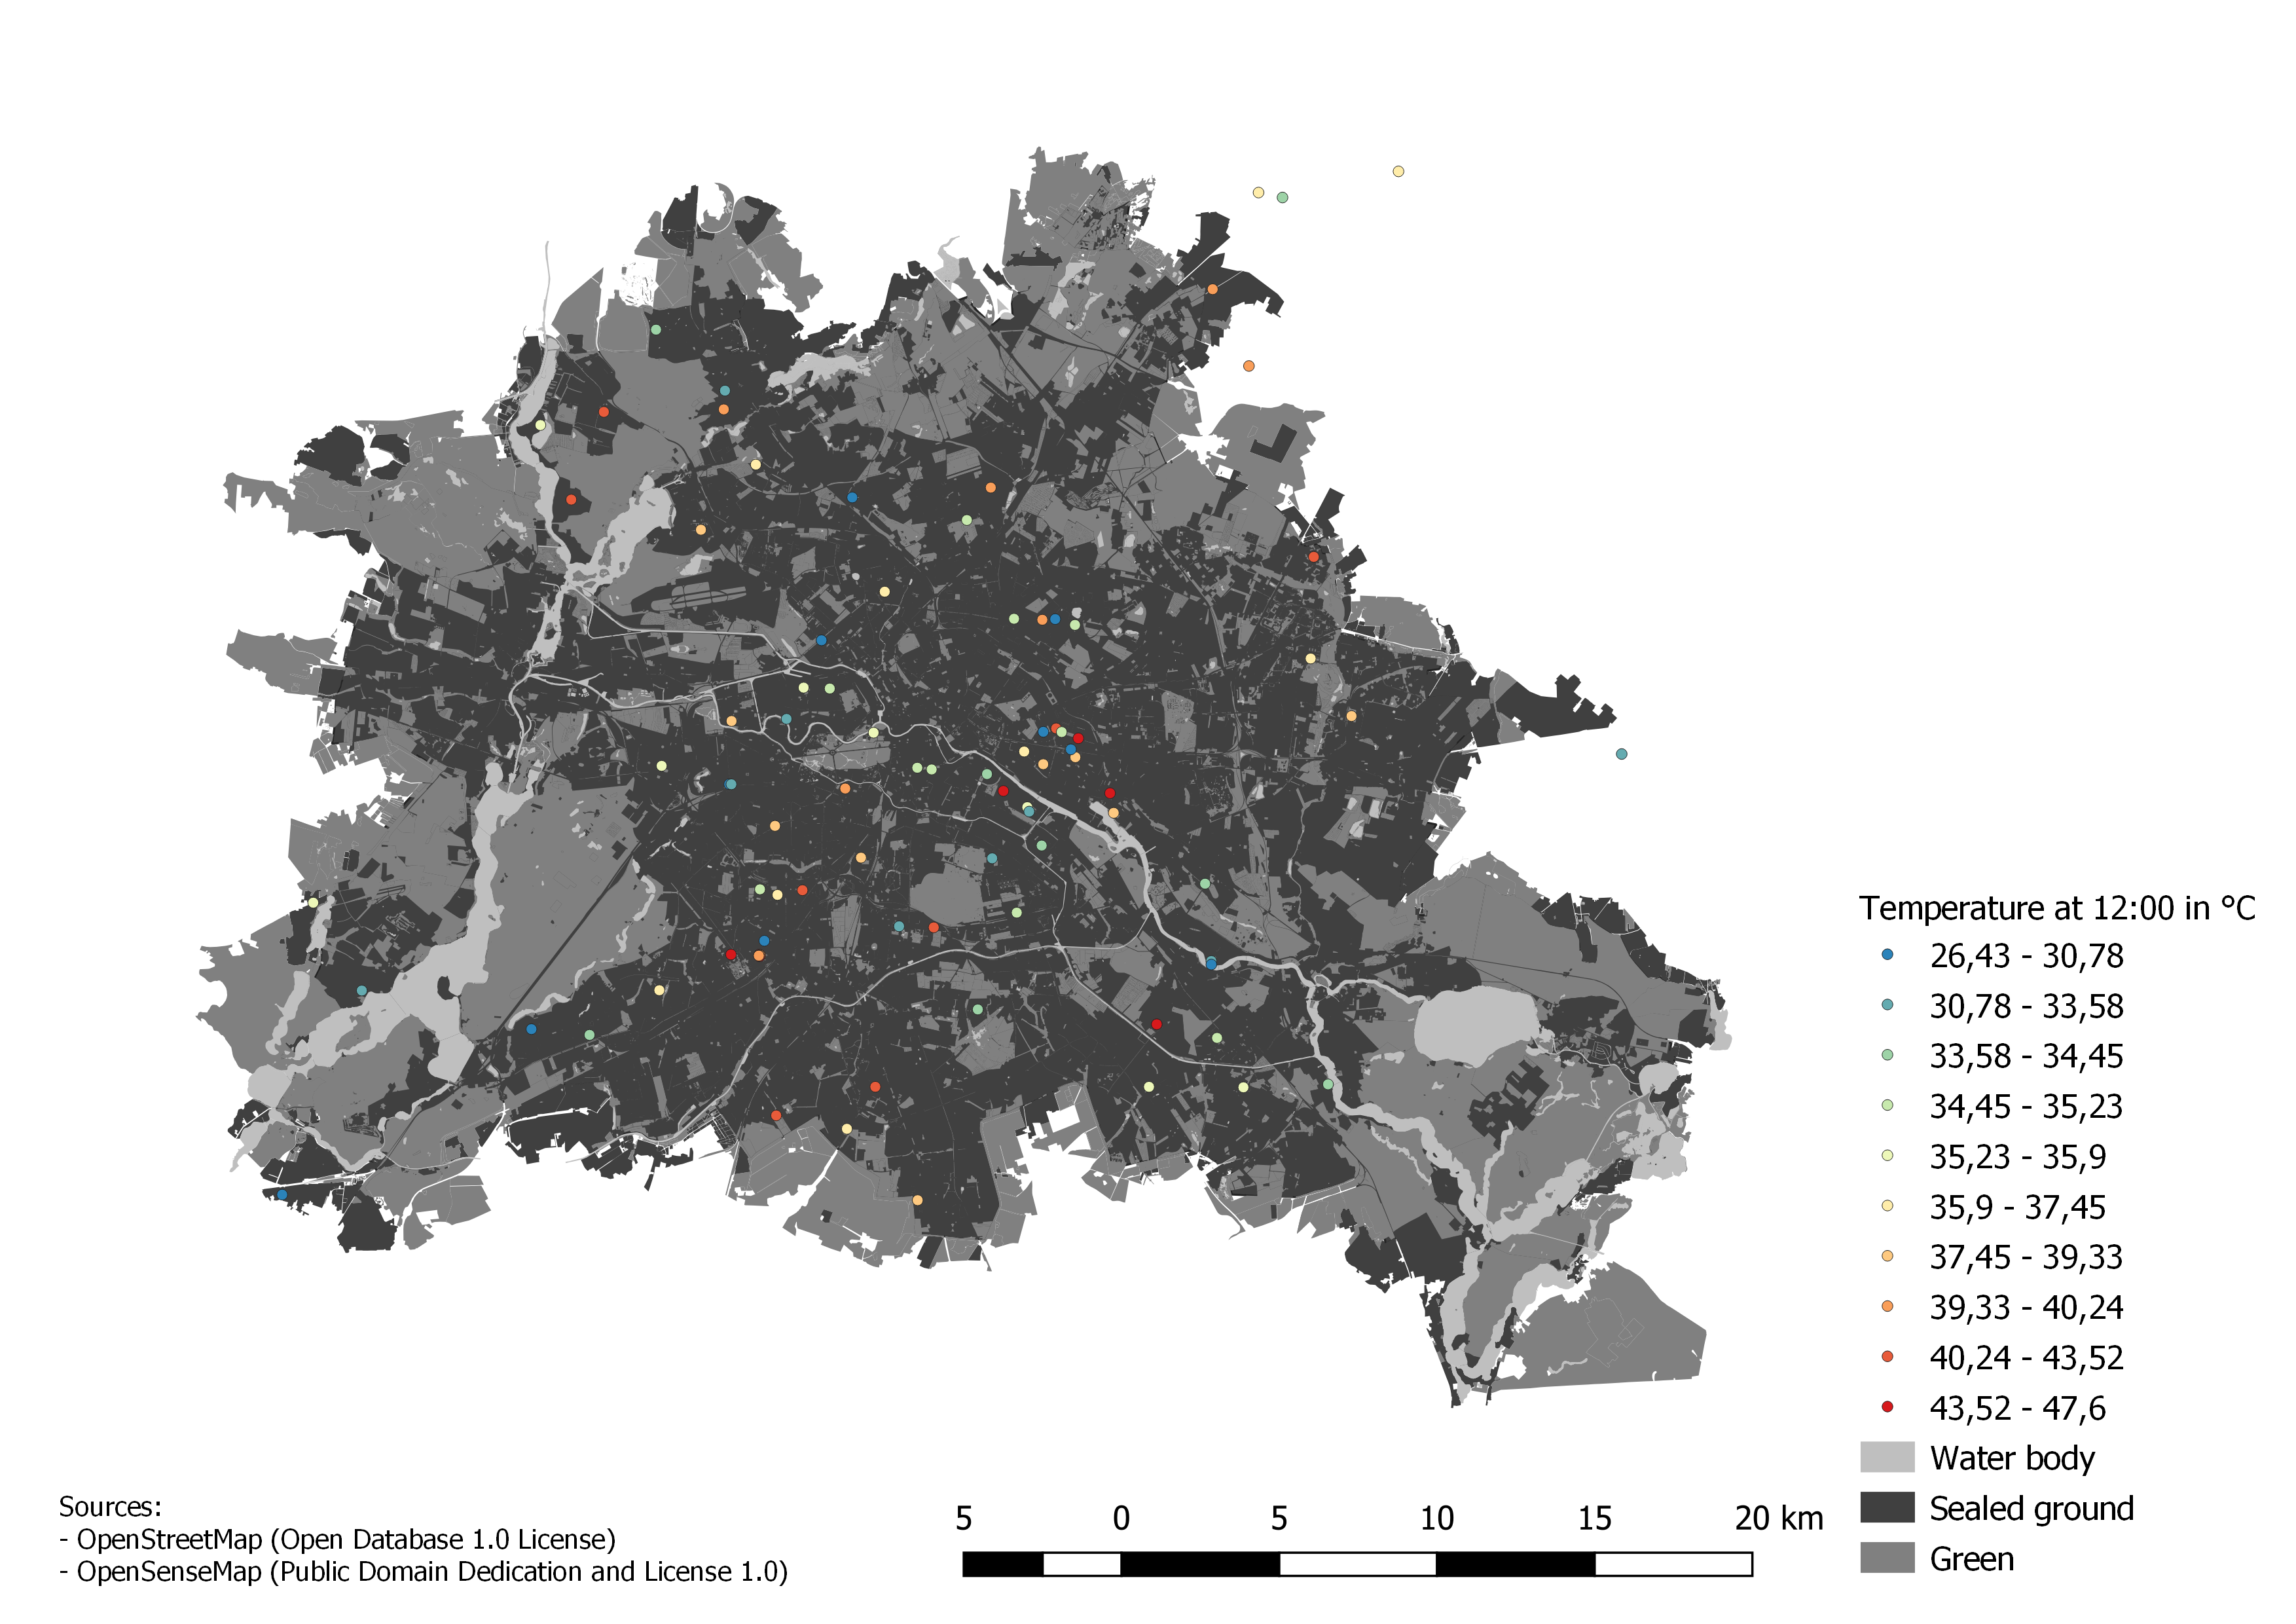
\includegraphics[width=\linewidth]{comparison/berlin.png}
	\caption{Surface types and sensor locations in research area}
	\label{fig:result_berlin}
\end{figure}

\subsection{Nearest neighbor}

The method \ldq{}nearest neighbor\rdq{} is displayed by smaller regions (cells) with sharp edges  (see figure \ref{fig:result_nearest}). Its distinctive visual characteristics do no give sophisticated information about the temperature distribution within the city of Berlin. The geometric shapes of the regions only give a general idea of where the heat islands are, but it does not allow a detailed analysis of the effect nor give a precise location/center of the heat.

\begin{figure}
	\centering
	\subfloat[\centering Nearest neighbor interpolation using GDAL\label{fig:result_nearest}]{{\includegraphics[width=.48\linewidth]{images/interpolation_nearest.png} }}
	\hfill
	\subfloat[\centering TIN interpolation using GDAL\label{fig:result_linear}]{{\includegraphics[width=.48\linewidth]{images/interpolation_tin.png} }}
	\caption{Nearest neighbor and TIN interpolation using GDAL in comparison}
	\label{fig:result_nearest_linear}
\end{figure}


\subsection{TIN interpolation}

Figure \ref{fig:result_linear} shows the TIN interpolation. Hereby visible is the characteristic surface made of triangles and the sharp edges. Due to visual examination the underlying calculation based on the relationship with the nodes of the triangles are apparent. The IUHI is not sufficiently depicted and is not very detailed and therefore does not provide enough information. The fact that TIN interpolation was used to create the image can easily be seen due to the visible convex hull.


\subsection{IDW interpolation}

For the IDW interpolation, GDAL and GRASS GIS were used in order to be able to compare the results. Visually, IDW is recognizable by the \ldq{}Bull Eyes\rdq{}-effect. These are concentric areas of equal values, which ​can be seen around the known points or stations. Compared to th nearest neighbor and TIN interpolation methods, IDW gives a much more detailed output and allows for distinctive analysis of the temperature distribution. Both results calculated with GDAL and GRASS give similar results as shown in figure \ref{fig:result_idw_gdal_grass}. Although the prominent points are fairly similar, differences can be seen in more sparsely covered areas.

\begin{figure}
	\centering
	\subfloat[\centering IDW interpolation using GDAL\label{fig:result_idw_gdal}]{{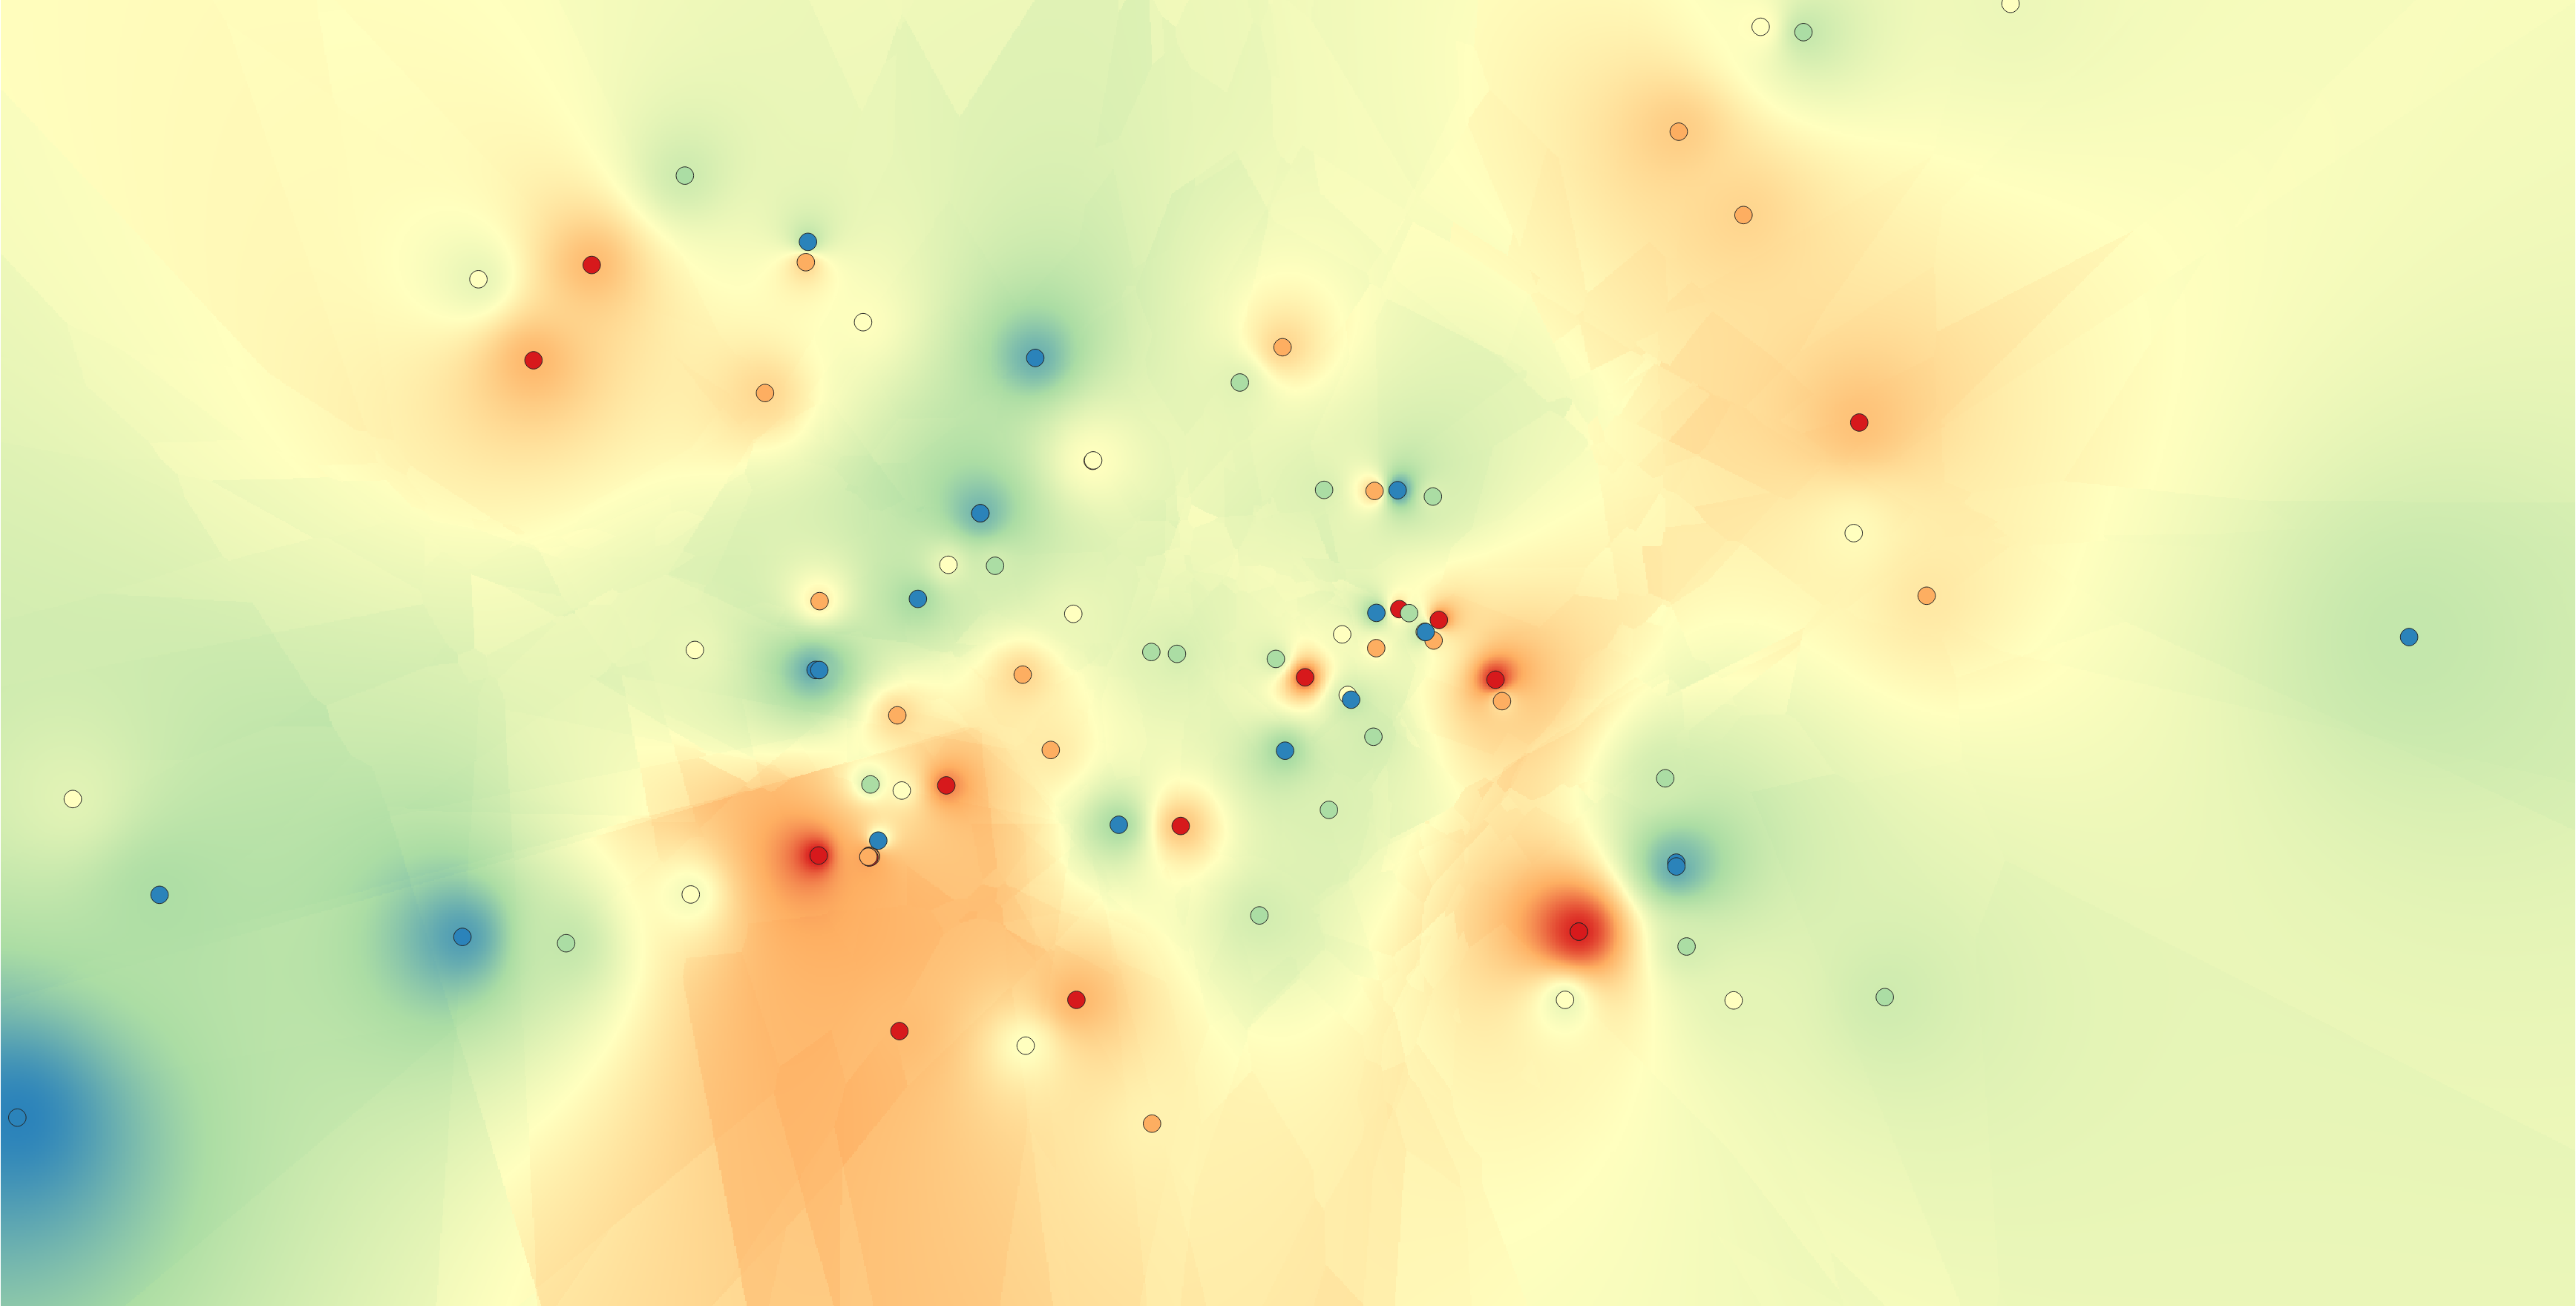
\includegraphics[width=.48\linewidth]{comparison/compare_idw_gdal.png} }}
	\hfill
	\subfloat[\centering IDW interpolation using GRASS GIS\label{fig:result_idw_grass}]{{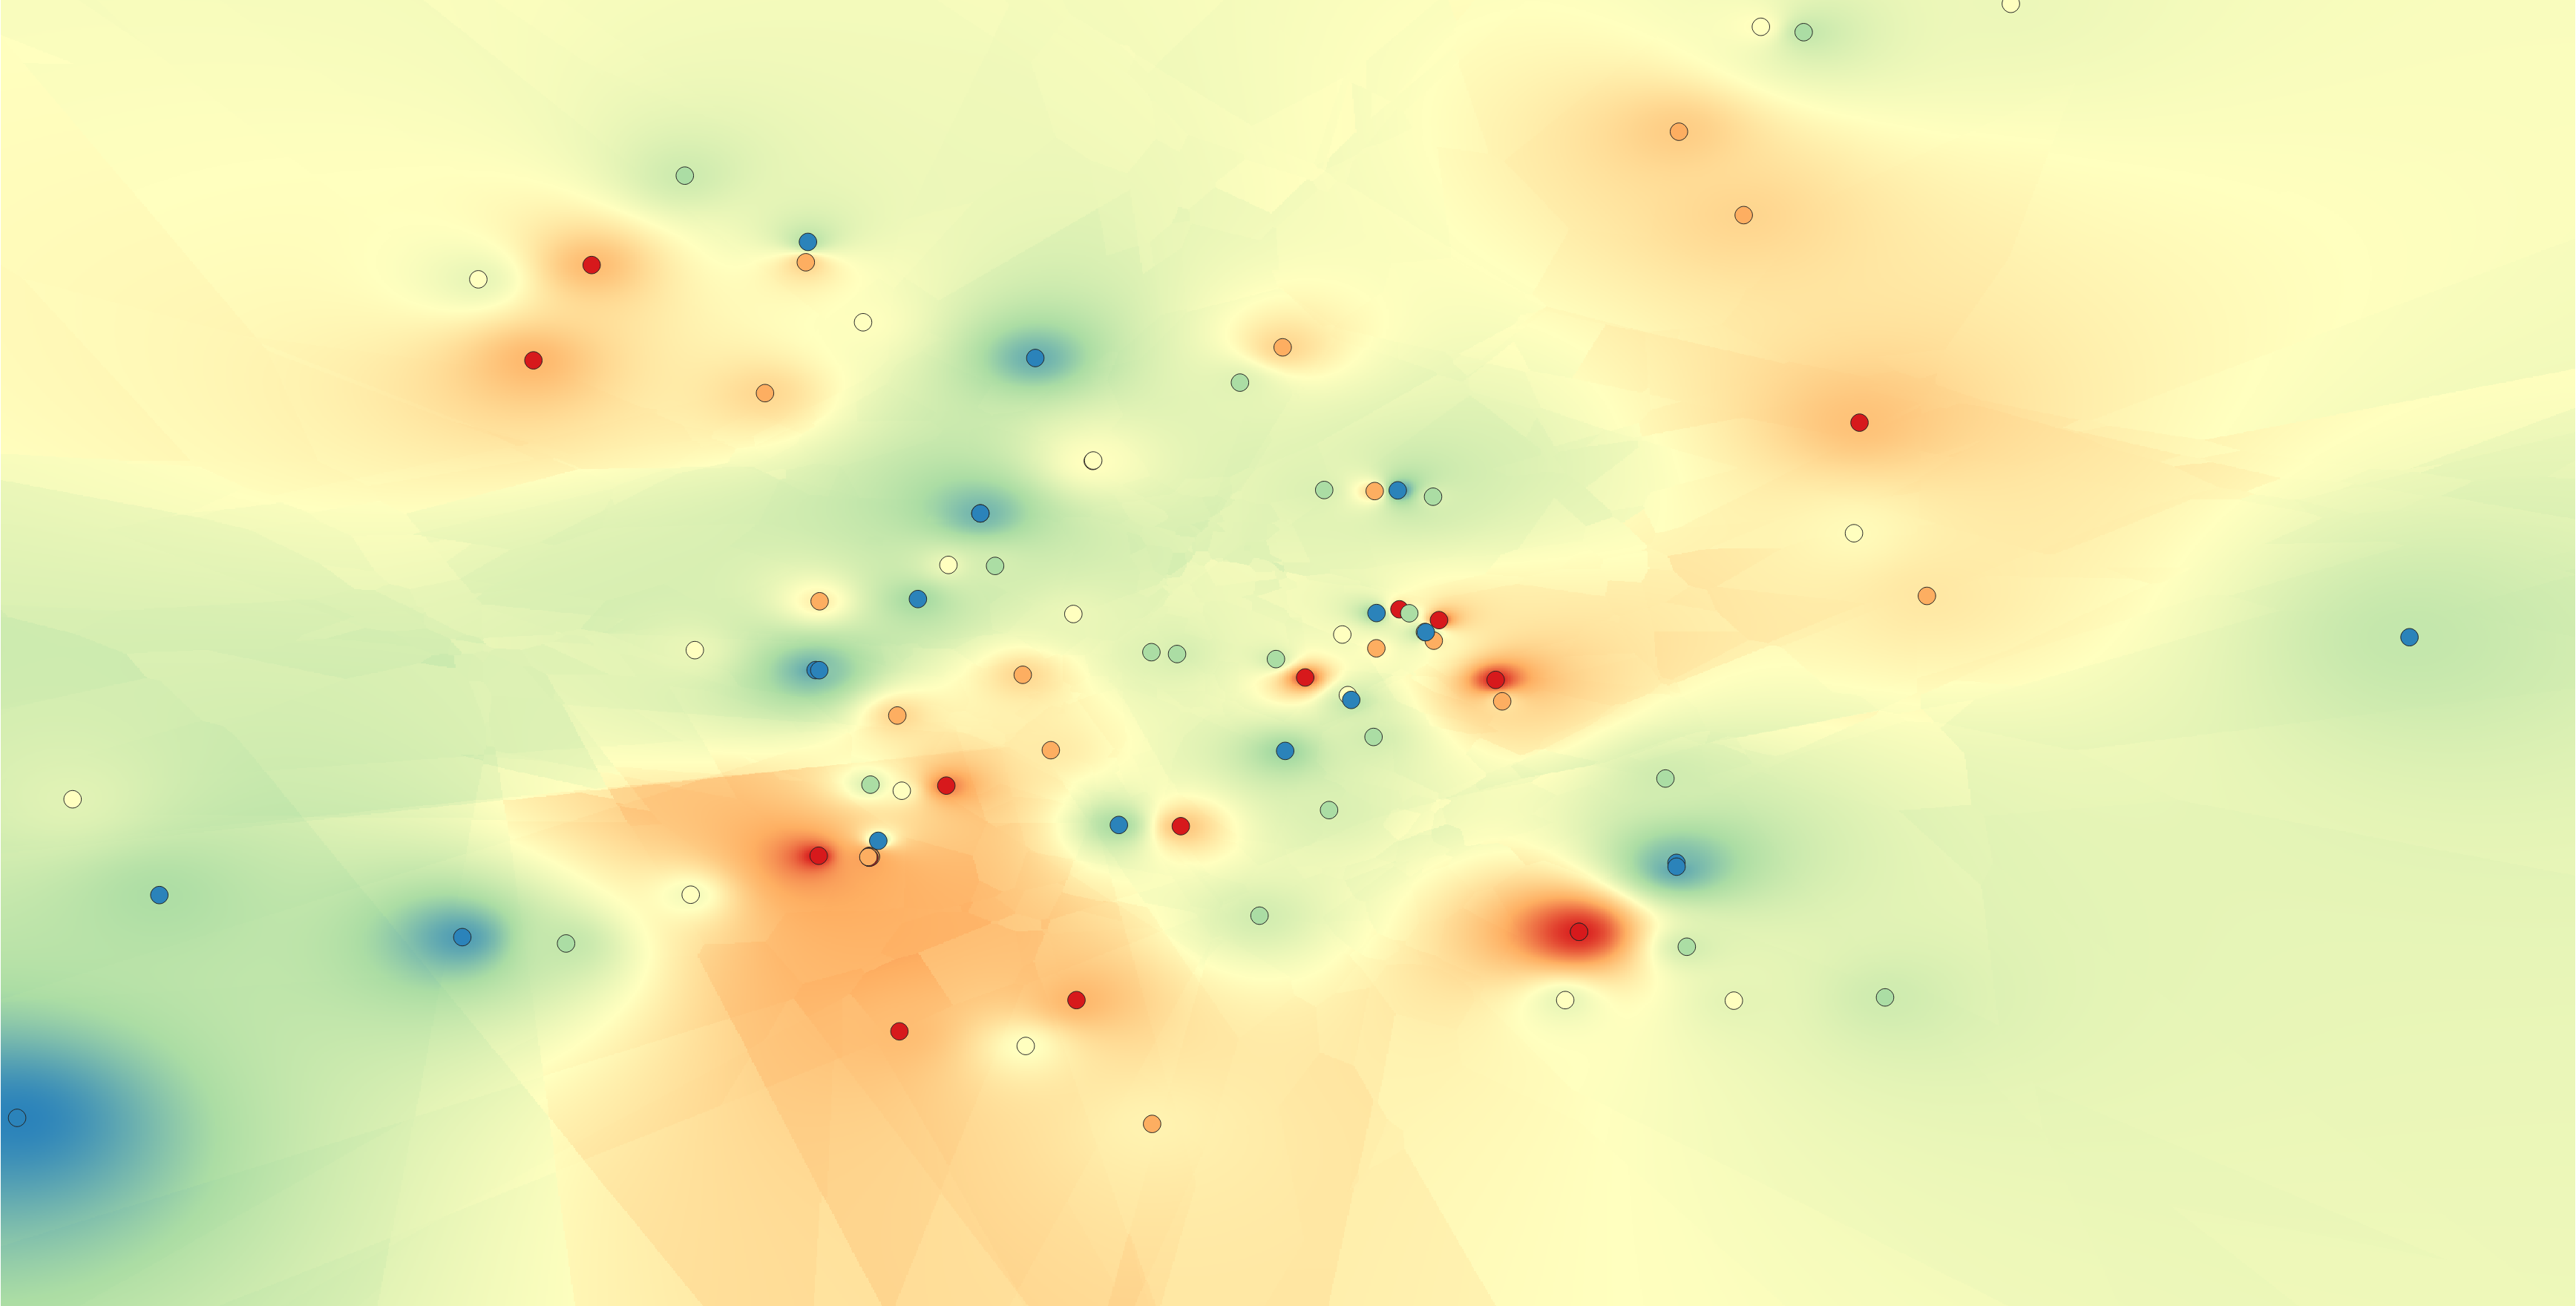
\includegraphics[width=.48\linewidth]{comparison/compare_idw_grass.png} }}
	\caption[Comparison of IDW interpolation between GDAL and GRASS GIS]{Comparison of IDW interpolation between GDAL and GRASS GIS, both using 12 max neighbors and a power factor of 2}
	\label{fig:result_idw_gdal_grass}
\end{figure}

\subsection{B-Spline interpolation}

As SAGA GIS also offers the possibility to interpolate point data, we conducted a B-Spline approximation. SAGA was identified as being one of the least accurate methods as illustrated by \citeauthor{wenjing_cao_study_2009}. As argued before, data points, which are not evenly distributed and have large value differences could pose a problem for spline interpolation. The result seems to have been \ldq{}smoothed\rdq{} out heavily and thus display a very homogeneous data surface. Figure \ref{fig:result_bspline} show that temperature distributions have farther reaching impact (compare lower left corner as well as the rightmost station with IDW). The smoothness can be seen on multiple clusters where the IDW interpolation creates islands that aren't interconnected and have more fringed edges.

\begin{figure}[H]
	\centering
	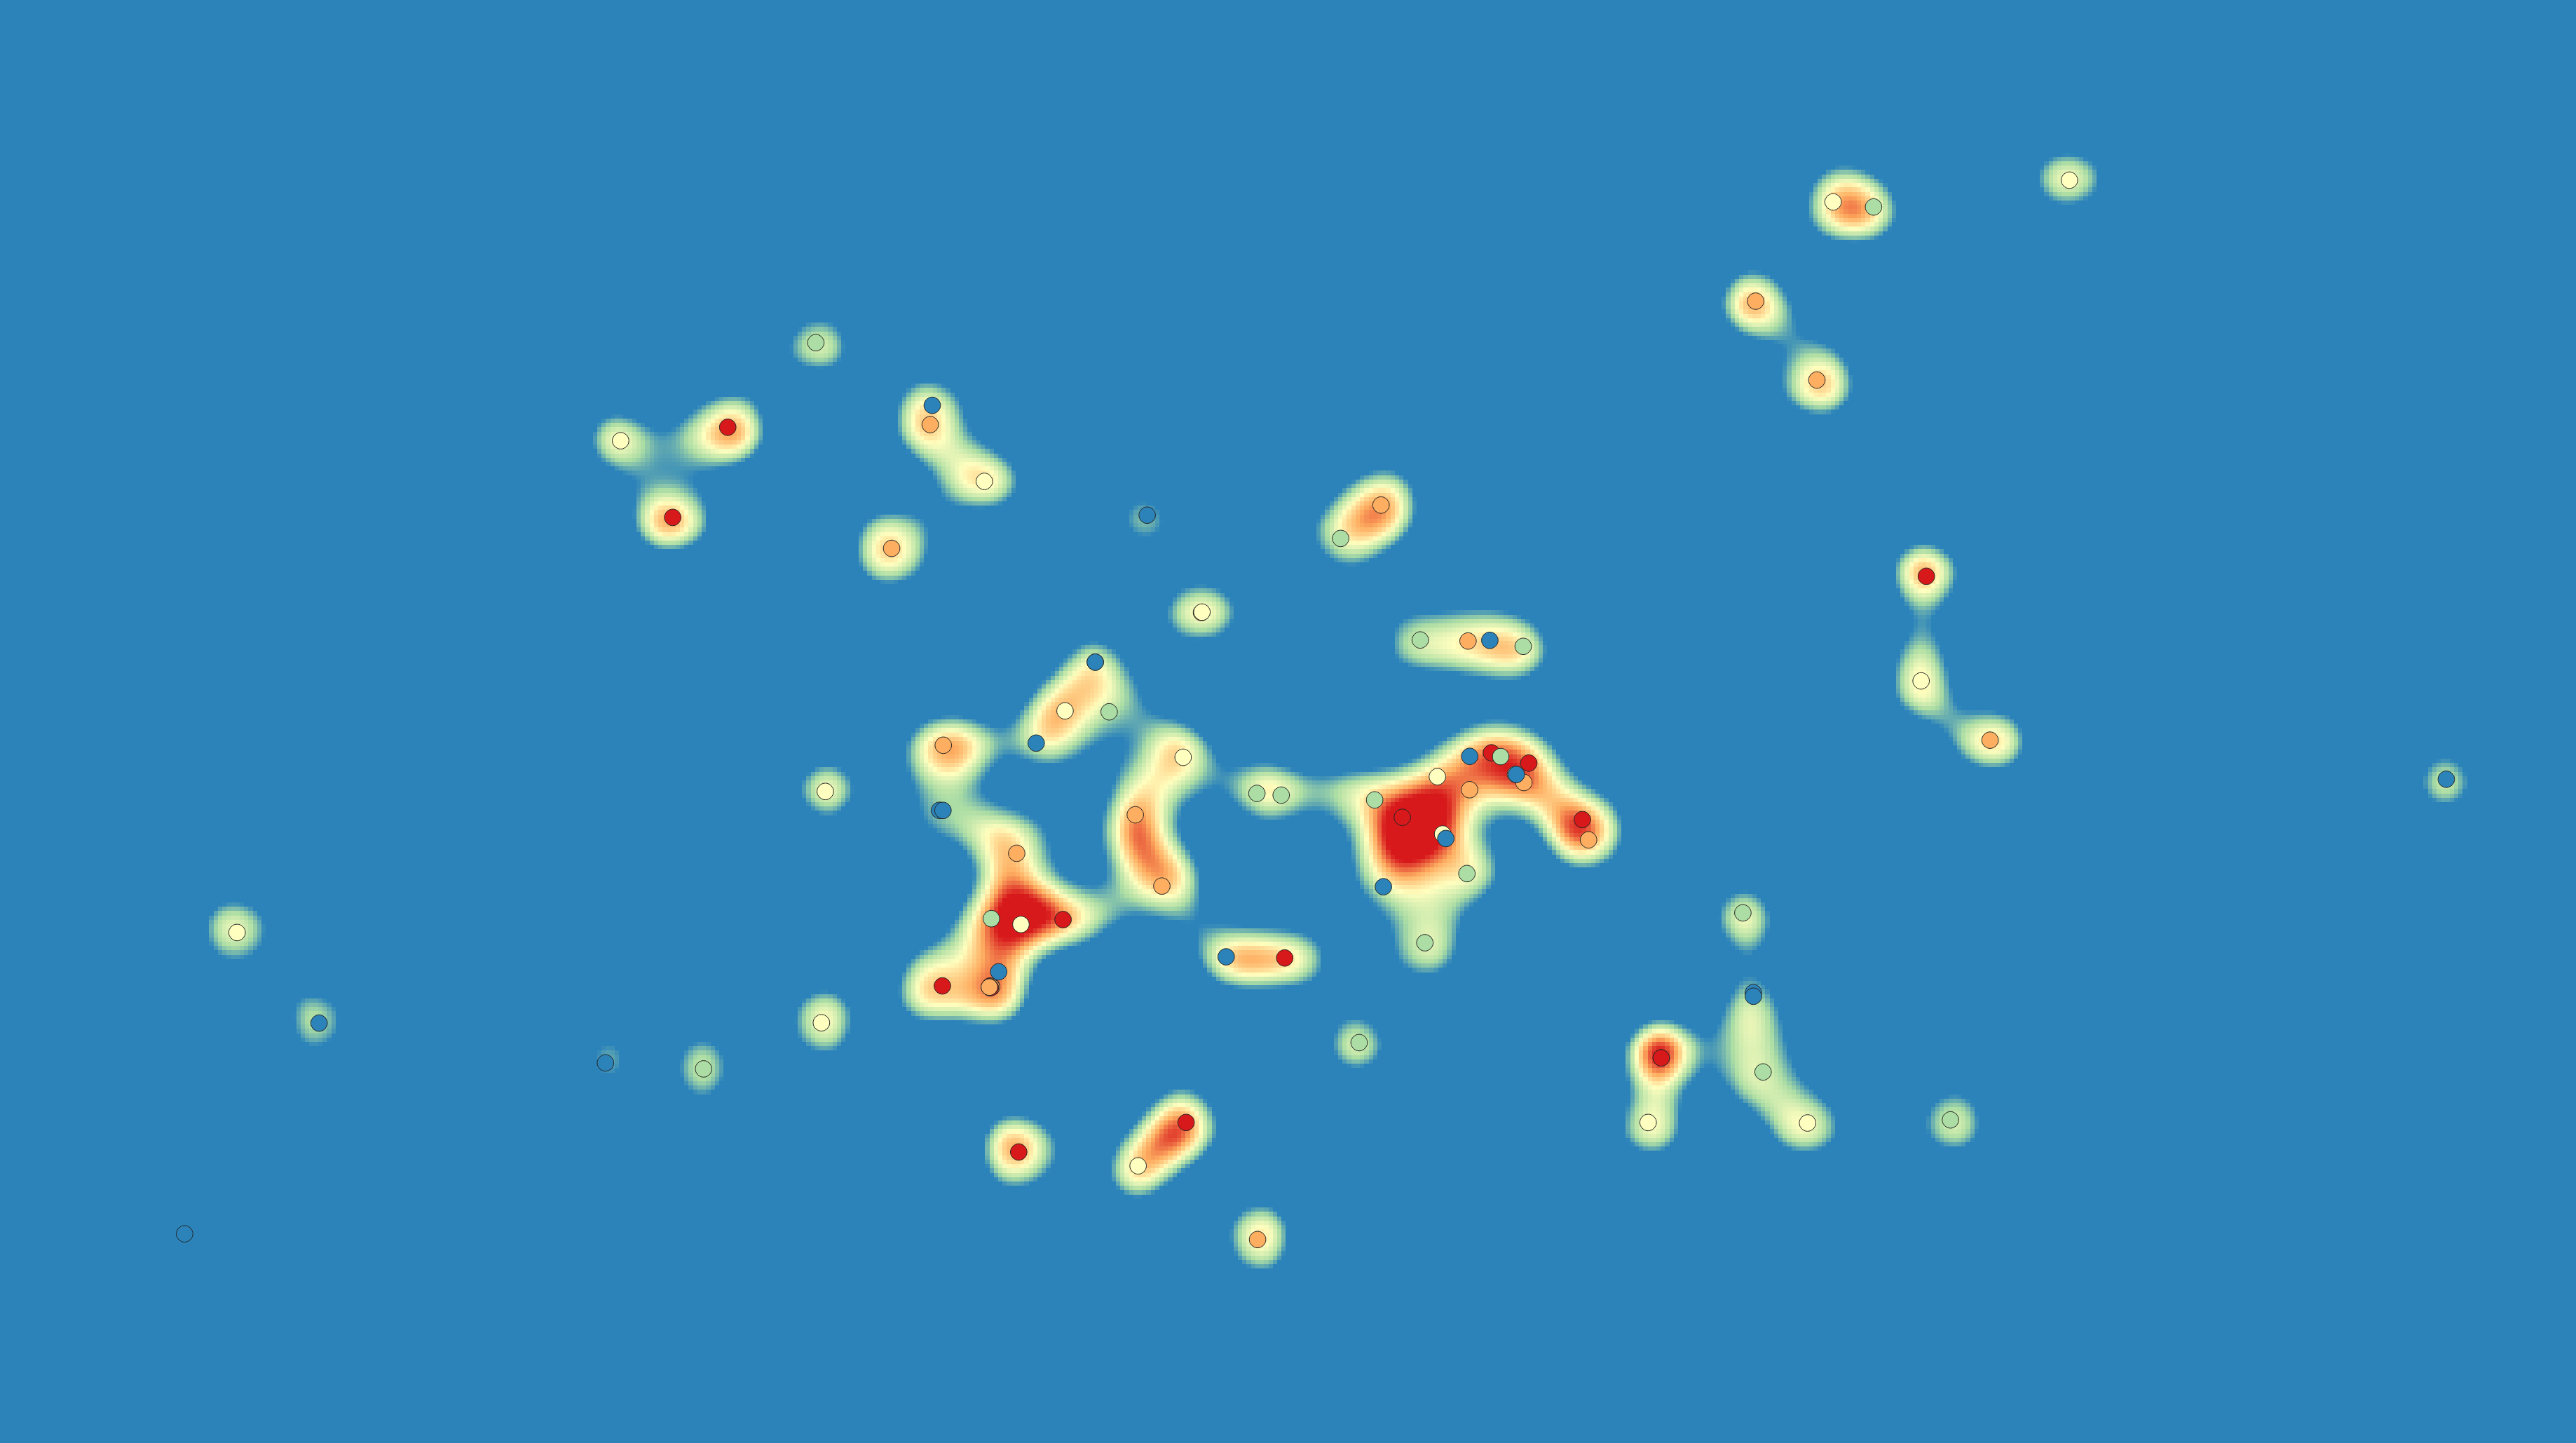
\includegraphics[width=.7\linewidth]{comparison/compare_bspline_saga.png}
	\caption{B-Spline interpolation using SAGA GIS}
	\label{fig:result_bspline}
\end{figure}

	
	\include{content/outlook}
	
%	{
%		\metroset{sectionpage=none,numbering=none}
%		\section{Demo}
%		\begin{frame}[standout]
%			\begin{env}
%				\usebeamercolor[fg]{normal text}
%				\LARGE
%				DEMO
%			\end{env}
%		\end{frame}
%	}

	\include{content/appendix}
	
\end{document}
